
\section{Chapter 2:\\ Paleorecords reveal biological mechanisms crucial for reliable species range shift projections amid rapid climate change}
\label{chapter2}

\vspace*{1cm}
\sffamily
\large
\begin{center}
Victor Van der Meersch$^1$, Edward Armstrong$^2$, Florent Mouillot$^1$, Anne Duputié$^3$, Hendrik Davi$^4$, Frédérik Saltré$^5$, Isabelle Chuine$^1$

\vspace*{0.1cm}
\small
\emph{$^1$CEFE, Univ Montpellier, CNRS, EPHE, IRD, Montpellier, France\\}
\emph{$^2$Dept. of Geosciences and Geography, University of Helsinki, Helsinki, Finland\\}
\emph{$^3$UMR 8198-EEP-Evo-Eco-Paleo, Université de Lille, CNRS, Lille, France\\}
\emph{$^4$URFM ,INRAE, Avignon, France\\}
\emph{$^5$Global Ecology, College of Science and Engineering, Flinders University, Adelaide, Australia}
\end{center}

\vspace*{0.7cm}
\normalsize
\textbf{Currently in review in \emph{Ecology Letters}. Preprint available here:\\} \url{https://doi.org/10.1101/2024.05.06.592679}

\vspace*{1cm}

\textbf{ABSTRACT}\\
The recent acceleration of global climate warming has created an urgent need for reliable projections of species distributions, widely used by natural resource managers. Such projections have been mainly produced by correlative species distribution models (CSDMs) with little information on their performances in novel climates. Here, we hindcast the range shifts of forest tree species across Europe over the last 12,000 years to compare the reliability of three different types of models. We show that the performance of CSDMs decreases twice as fast as that of process-explicit models (PEMs) when climatic dissimilarity rises, and that PEM projections are likely to be more reliable than those made with CSDMs, at least until 2060 under scenario SSP245. These results demonstrate for the first time the well-established albeit so far untested idea that explicit description of mechanisms confers model robustness, and highlight a new avenue to increase model projection reliability in the future.

\rmfamily

\newpage

\subsection{Introduction}\label{intro2}

% Modelling is essential for understanding and predicting  the impacts of  climate change on ecosystems and biogeochemical cycles. 
Credible model projections are critical for natural resource managers, decision makers and stakeholders to make informed decisions. To meet the demand for reliable projections of ecosystems and biodiversity dynamics, comprehensive assessments  of ecological model performances must be a priority \citep{Dawson2011, Mouquet2015, Pacifici2015}. 

One approach to evaluate model reliability is to compare their predictions to observations from previous time periods, i.e. hindcasting. Hindcasting can inform whether models capture, implicitly or explicitly, the essential processes required to provide reliable projections in conditions significantly different from the present. By looking far into the past, paleo-archives have proven to offer a unique opportunity to both understand long-term climate and biodiversity dynamics \citep{Bartlein2011, Fordham2020} and test model robustness and transferability (i.e. model capacity to maintain its performance in changing conditions; \citealp{UribeRivera2023}) \citep{Braconnot2012, Maguire2015}.  

Yet, models prediction of past species distribution and biospheric components have rarely been consistent with paleoclimate reconstructions and fossil records \citep{Veloz2012, Pearman2008b, Roberts2012, Foley2013, Maguire2016}. Interpreting model projections in climatic conditions that differ significantly from the present, such as future no-analogue climatic conditions \citep{Williams2007}, remains challenging. Therefore, the guarantee that ecological model forecasts for the 21\textsuperscript{st} century will be reliable is limited \citep{Fitzpatrick2018}. 

While exact matches to expected 21\textsuperscript{st}-century climatic conditions do not exist in historical records \citep{Burke2018}, the dissimilarity between 20\textsuperscript{th} and 21\textsuperscript{st} century median climatic conditions (\hyperref[methods2]{Methods}) falls within the range of dissimilarity encountered since the beginning of the Holocene (12 kyr BP, with kyr = 1000 years and BP = Before Present (1950); \Cref{fig:climaticdissimilarity}). This period takes place after the Last Glacial Maximum (26.5-19 kyr BP; \citealp{Clark2009}) and began with an abrupt climate warming followed by a long, almost uninterrupted, period of climatic stability until recent anthropogenic warming (\Cref{fig:S1}). The fossil pollen data accumulated over these last millennia provides us with an unique extended timeframe to test the reliability of ecological models, in particular those designed to predict changes in species distribution.

\begin{figure*}[ht!]
\centering
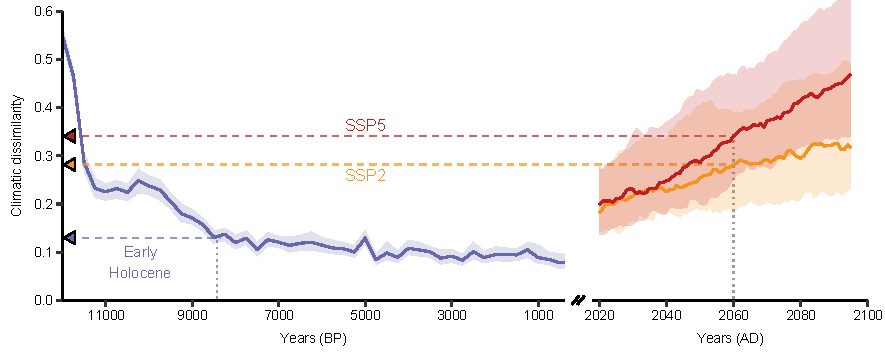
\includegraphics[width=17cm]{chapter2/figs/climatic_dissimilarity.pdf}
\caption{\textbf{Evolution of climatic dissimilarity during the Holocene (12k-500 yr BP) and the 21\textsuperscript{st} century (2005-2100), relative to 1901-2000.} Climatic dissimilarity is computed as 1-Sørensen similarity between bootstrapped climatic hypervolumes. Lines represent median dissimilarity, shaded areas represent 90\% confidence intervals. Blue corresponds to paleoclimate based on HadCM3B model. Yellow and red correspond to future climatic conditions according to SSP245 and SSP585 scenarios respectively, predicted by 34 global climate models of NEX-GDDP-CMIP6. The blue triangle on y-axis indicates the level of climatic dissimilarity 8500 years ago, at the limit between the Early and Late-Middle Holocene. Yellow and red triangles indicate the expected level of climatic dissimilarity in 2060 for SSP245 and SSP585 scenarios. Note that the x-axis scale is different between past and future panels.}
\label{fig:climaticdissimilarity}
\end{figure*}

Species distribution models are powerful tools to predict species geographical distribution as a function of environmental data (e.g., mean annual temperature and annual total precipitation). Most studies have focused on correlative species distribution models (CSDMs, or niche models), which infer statistical relationships between observations of species occurrences and environmental predictors \citep{Dormann2012}. Their high flexibility and low computational complexity make them the most widely used tool for deciding on species conservation plans and policy regimes \citep[e.g.][]{Hanewinkel2013}. However, under novel climatic conditions, new unobserved portions of a species’ climatic niche may appear, which are not captured by these correlative (or phenomenological) approaches. For example, when tested under distant past climates, the predictive performance of CSDMs  significantly decreased \citep{Maguire2016}, questioning their ability to provide reliable projections in the future \citep{Fitzpatrick2018}. However, these discrepancies might be partly due to dispersal constraints which can create a disequilibrium between species distribution and climate \citep{Svenning2004}.

Alternative approaches to CSDMs are process-explicit models (PEMs, or process-based models) that rely on explicit formulations of the mechanisms driving the distribution of a given species (e.g., physiological, ecological and/or demographic processes). They come from decades of experiments and observations, including extreme conditions in laboratory \citep{Seehausen2017}, and climate manipulations such as CO\textsubscript{2} enrichment \citep{Jiang2020} or rainfall exclusion \citep{Gavinet2019}. The reliability of PEMs depends on our level of understanding of how environmental conditions affect ecophysiological processes, and the availability of large amount of observations to calibrate their many parameters \citep{Evans2016}. Because these models do not rely on statistical relationships between present-day species occurrences (presence/absence) and environmental variables, but rather describe explicit causal relationships between biological processes and environmental variables, they are believed to provide more reliable predictions of species distribution changes under novel climatic conditions  \citep{Evans2012, Singer2016}. However, another possible reasons why PEM projections might be more reliable than CSDM projections under novel climatic conditions could also come from their calibration methods. Unlike CDSMs that are calibrated using species presence/absence data, PEM parameters are either measured directly (e.g. specific leaf area, leaf frost hardiness), or inferred statistically when direct measurement is not an option, using data on specific functional traits measured in the field or in laboratory (e.g. parameters of bud dormancy break date models). 

% Despite the growing interest for PEMs in predictive ecology \citep{Evans2012, Connolly2017, Urban2016, Pilowsky2022}, the widespread assumption that they provide more reliable projections of future species range shifts has yet to be verified. 
The assumption that PEMs could provide more reliable projections of future range shifts of species is widely accepted and taken for granted \citep{Evans2012, Connolly2017, Urban2016, Pilowsky2022} although it has never really been demonstrated.
Furthermore,  the reasons behind this assumption have not been clearly articulated. Qualitative models comparison under future climatic conditions have shown that PEMs often make more conservative projections in future climates than CSDMs which predict larger changes \citep{Morin2009, Cheaib2012, Gritti2013} but they have not provided any confidence level in these results. Very few studies have actually gone beyond qualitative comparisons between CSDMs and PEMs and compared thoroughly their performance, for example using virtual species \citep{Zurell2016}, exotic species in native and newly colonized areas \citep{Higgins2020}, or in the recent past \citep{Fordham2018}. 
While PEMs have shown their usefulness for paleoecological studies \citep{Saltre2013, Ruosch2016, Schwoerer2014}, the extent to which they can provide more reliable predictions than CSDMs under different climatic conditions from the historical period remains unknown \citep{UribeRivera2023, Briscoe2019}. 

Here, we address this critical gap by using multiple CSDMs and PEMs to simulate paleodistributions of five emblematic tree species of Europe at a high temporal resolution since 12 kyr BP. We used daily paleoclimatic data at 0.25° spatial resolution, generated from HadCM3B-M2.1 coupled general circulation model simulations, which includes both inter-annual variability, and millennial scale variability for rapid Dansgaard–Oeschger events before 11 kyr BP \citep{Armstrong2019}. Species migration ability was also incorporated into the simulations to represent more comprehensively changes in species' realized distribution and not merely changes in their climatic niches to allow for a more  accurate comparison with the paleorecords.

We first assessed which modelling approach best predicts past species distributions, and second whether model performance was related to their hypotheses (relationships describing explicit biological mechanisms or not) or to their calibration methods (calibrated on species occurrence data or not). To do so, we compared three types of models: CSDMs, PEMs (hereafter called expert PEMs) and fitted PEMs calibrated in the same way as CSDMs (inverse calibration using species occurrence data and a novel type of algorithm; \hyperref[methods2]{Methods}; \citealp{VanderMeersch2023}). The comparison between CSDMs/fitted PEMs and expert PEMs allowed us to determine whether the differences in model performance arise from their calibration methods, whereas the comparison between CSDMs and expert/fitted PEMs allowed us to determine whether the differences in model performance arise from the model hypotheses. We assessed the performance of the models for the maximum level of climate dissimilarity possible, i.e. over the last 12,000 years, which corresponds to the climate dissimilarity expected by the end of the century according to SSP245, and by the middle of the century according to SSP585 (\Cref{fig:climaticdissimilarity}).

\subsection{Methods}\label{methods2}

\subsubsection{Correlative and process-explicit species distribution models}\label{models}

We used PHENOFIT and CASTANEA, two process-explicit models which differ by their underlying hypothesis and complexity. PHENOFIT simulates the fitness of an average adult tree \citep{Chuine2001}. It estimates fitness components (survival and reproductive success) by simulating the precise phenology (dates of leaf unfolding, flowering, fruit maturation, leaf senescence) and damages caused by abiotic stress (frost, drought) which effects depend on their occurrence relatively to the development stages of the different organs. It has been validated for several North American and European species \citep{Morin2007, Saltre2013, Duputie2015, Gauzere2020}. The model has \textappr30 parameters. CASTANEA simulates carbon and water cycles of an average adult tree by simulating many processes such as photosynthesis, stomatal opening, maintenance and growth respiration, transpiration and carbon allocation  \citep{Dufrene2005}. It has been used to predict carbon and water budgets of several European species \citep{Davi2006, Delpierre2012, Davi2017}. The model has \textappr80 parameters. Both models require daily meteorological variables and soil characteristics. Two versions of both models were employed: one was calibrated with expert knowledge and statistical inference using observations and measurements of the processes modelled (version called \emph{expert}), and a second one was entirely calibrated using species distribution data (version called \emph{fitted}; \citealp{VanderMeersch2023}) like correlative models. For the latter, we used the optimization algorithm CMA-ES \citep{Hansen2001} as described in \citep{VanderMeersch2023}, and retained the best calibrations in terms of AUC.
  
We selected correlative models based on the thorough model comparison made by \cite{Valavi2022}. Among the most performant models, we selected five well-established models: GLM with lasso regularization, GAM, BRT, MaxEnt and down-sampled Random Forest. Some of these models are known to struggle when applied to extrapolation domains, but are nevertheless widely used by ecologists to provide projections of species distribution change in future climatic conditions.
We chose four uncorrelated climate predictors related to ecological processes to calibrate these models: minimum temperature of the coldest month (representing frost tolerance), total precipitation (representing available water), GDD5 (growing degree days  \textgreater5°C) between April and September (representing available thermal energy for vegetation growth and fruit maturation), water balance between June and July (precipitation$-$evapotranspiration, representing summer drought tolerance). We also included two soil covariates (pH and Water Holding Capacity).
  
While by construction correlative models directly output species habitat suitability, we used fitness predicted by the model PHENOFIT and net primary production predicted by the model CASTANEA as a proxy of species habitat suitability as they have already been used to predict species presence in previous studies \citep{Morin2009, Cheaib2012, Saltre2013}. CSDMs and inverse-calibrated PEMs were calibrated for five species (\textit{Fagus sylvatica} L., \textit{Abies alba} Mill., \textit{Quercus robur} L., \textit{Quercus petraea}  (Matt.) Liebl. and \textit{Quercus ilex} L.) using historical climate (1970-2000) extracted from ERA5-Land hourly dataset \citep{MunozSabater2021}, soil data from EU-SoilHydroGrids \citep{Toth2017} and SoilGrids \citep{Hengl2017} databases and species presence data from the dataset assembled in \cite{VanderMeersch2023}, mostly based on EU-Forest inventory data \citep{Mauri2017}. To calibrate the CSDMs, we additionally sampled 50,000 background points, which should properly represent the variation in the environmental conditions across the study area \citep{Valavi2022}. For each CSDM and each species, we run a fivefold environmental cross-validation to estimate model performance in novel extrapolation conditions (\Cref{fig:S8}; \citealp{Roberts2017}). We then used all the available training data to calibrate the models for the hindcasting in order to favour final prediction quality \citep{Roberts2017}. We could not run the same cross-validation method for fitted process-explicit models because it would have been too computationally expensive. 

Model simulations over the Holocene were run for 30-year periods every 250 years, for the five above mentioned species. Model outputs were averaged over each 30-year period. Note that soil conditions (needed both for correlative and process-explicit models) were held constant throughout the simulations, and were bilinearly interpolated from closest coastal cells where data was missing (because of different land-sea masks between present and past). Note also that for CASTANEA model, species-specific thresholds of net primary production determining the presence or absence of the species were computed with the CO$_2$ level at the beginning of the Holocene (\textappr240ppm).

\subsubsection{Late Quaternary climate and vegetation}\label{paleodata}

We used the monthly paleoclimate simulation dataset generated with the HadCM3B-M2.1 coupled general circulation model \citep{Armstrong2019}, starting from 18 kyr BP at 0.5\degree~spatial resolution for Europe (\Cref{fig:S1}). We chose this dataset for several reasons. First, it includes both inter-annual variability, and millennial scale variability for rapid Dansgaard–Oeschger events before 11 kyr BP. Second, it shows generally a good agreement with ice-core datasets \citep{Armstrong2019}. Third, it provides all the necessary input variables necessary to run all the models selected.  For this work, several variables were specifically produced: mean temperature, average minimum and maximum daily temperatures, precipitation, number of rainy days, cloudiness, and wind speed. We further downscaled temperature and precipitation monthly data to 0.25\degree~resolution, by applying an elevation correction of coarse-scale variables towards the ICE-6G-C elevation level at high resolution \citep{Peltier2015}.  
We then generated daily data for temperatures, precipitation, cloud cover and wind speed from  the monthly data with the weather generator GWGEN \citep{Sommer2017}, for 30-year periods every 250 years. We also simulated daily extra-terrestrial solar radiation with the same orbital forcing conditions used in HadCM3B-M2.1 \citep{Armstrong2019} and then computed daily global radiation taking into account previously generated daily cloud-cover data as implemented in LPJ-LMfire global model \citep{Pfeiffer2013}. Finally, we computed daily potential evapotranspiration following the standard FAO Penman-Monteith method \citep{Allen1998}. Note that for smaller plants and shrubs, such macroclimatic variables may overestimate species range shifts \citep{Maclean2023}. The workflow used to downscale and generate daily climatic variables is summarized in the \Cref{fig:workflow}.

Fossil pollen records were extracted from the LegacyPollen dataset \citep{Herzschuh2022}. This dataset is mainly based on the Neotoma database \citep{Williams2018}, and provides samples with standardized chronologies and age uncertainties. We removed sites that had marine depositional environments \citep{Maguire2016}, and only kept samples with more than 200 pollen grain counts and age uncertainty of less than 500 years.
Pollen relative abundances were aggregated to consecutive 500-year intervals. If multiple samples from the same site belonged to the same period, we averaged their pollen abundances, weighting by their age uncertainty and temporal distance from the center of the period. Relative pollen abundances were converted to presence/absence using thresholds based on biome reconstructions \citep{Williams1998}: 1\% for \emph{Fagus} and \emph{Abies}, and 2.5\% for \emph{Quercus}. If several sites fell within the same grid cell (0.25\degree), we considered the species as present if there was at least one site where the species could be considered as present. \textit{Fagus} pollen data were used to assess the presence of \textit{Fagus sylvativa} L., sole species of the genus present in Europe. \textit{Abies} pollen data were used to assess the presence of \textit{Abies alba} Mill., most abundant and widespread fir species present in Europe. When possible, deciduous and evergreen \textit{Quercus} pollen were distinguished based on Neotoma data. Some \textit{Quercus} pollen remain undetermined beyond the generic level, either because discrimination between evergreen and deciduous oak pollen was impossible or because authors were not specific. They were assigned to two categories, based on the evergreen natural range as defined by Atlas Flora Europeae \citep{AFE2005} and EuroVegMap \citep{EVM2003}: pollen outside range were considered as deciduous only occurrences, whereas pollen inside range were considered as both evergreen and deciduous occurrences. Deciduous \textit{Quercus} pollen data were used to assess the presence of \textit{Quercus} \textit{petraea}  (Matt.) Liebl., and \textit{Quercus robur} L., the two most abundant and widespread deciduous oak species in Europe. Evergreen \textit{Quercus} pollen data were used to assess the presence of \textit{Quercus ilex} L., the most abundant and widespread evergreen oak species in Europe.

\subsubsection{Tree migration}\label{migration}

Models used in this study predict species potential distribution based solely on climatic and soil conditions. To compare model predictions to pollen paleorecords, species migration needs to be simulated as well, as it can be the primary factor limiting species distribution before climatic conditions, especially when climatic conditions are changing rapidly as it was the case during the Dansgaard–Oeschger events \citep{Svenning2004, Saltre2013}.

To implement migration in the simulations, we run a  cellular automaton \citep{Engler2012} which has proven to be as accurate as more complex approaches \citep{Zurell2016}. We modified the initial version of this dispersal model in order to use both short- and long-distance dispersal kernels (long distance events could occur with a probability of 0.01). We used species-specific fat-tailed kernels \citep{Zani2022} at a 500 m resolution, and assumed that trees can disperse once a year (\Cref{fig:S7}). Model outputs were assigned to two classes using specific optimal thresholds maximizing model performance (TSS) in the historical climate (\Cref{fig:S8}): (i) cells where the model output was under the specific threshold were assigned a zero suitability (species cannot survive), and (ii) cells where the  model output was above the threshold, the suitability was rescaled between 0 and 1 (species can migrate). We considered the deciduous \emph{Quercus} suitability as the maximum suitability between \emph{Q. robur} and \emph{Q. petraea}. Migration simulations started from 12 kyr BP (or 11.75 kyr BP when a model simulates no presence at 12 kyr BP). Note that starting at 11.75 kyr BP or 12 kyr BP does not change our results (\Cref{fig:S10}), and that we could not start earlier (e.g. \textappr15 kyr BP) as most models predict no presence at all around 12.5 kyr BP. We also checked that dispersal process stochasticity at 500m resolution (\Cref{fig:S7}) had no significant effect on the model's performance at the scale of Europe, by simulating deciduous \emph{Quercus} migration 10 times for each of the 8 models (\Cref{fig:S7}). 

\subsubsection{Models' performance}\label{skill}

We used the Sørensen's similarity index to measure the hindcast performance of the models, based on the confusion matrix. This discrimination measure has been shown to provide adequate estimations of model discrimination capacity,  not biased by species prevalence or an inflated number of true negative predictions \citep{Leroy2018}. This feature is important when working with fossil pollen data, for which the number of species absence can be much higher than the number of species presence. Note that we obtained similar results when using TSS as the performance metric (\Cref{fig:S10}). We compared the area potentially occupied (not taking migration into account) and occupied (taking migration into account) by the species to the presence/absence data extracted from the LegacyPollen dataset every 500-year interval. Kruskal-Wallis tests followed by multiple pairwise post-hoc Conover-Iman tests (as implemented in the R package \emph{conover.test}) were computed to assess stochastic dominance among model performance and transferability (\Cref{fig:pastperformance}).

To quantify the climatic differences between  historical climate (1901-2000, based on the CRU TS v. 4.07 gridded dataset; \citealp{Harris2020}) and Holocene climate (hindcasting conditions), we computed the \emph{climatic dissimilarity} as the Sørensen dissimilarity between climatic hypervolumes (a metric of overlap in multidimensional space). We first generated for each period (500-year intervals from -12 kyr BP to 500 BP and 1901-2000) a set of 20 bootstrapped hypervolumes, using R package \emph{hypervolume} \citep{Blonder2018}. Hypervolumes were computed with a Gaussian kernel density estimation method based upon the first three principal component axis from three-month means temperature and three-month sums of precipitation. We then computed overlap statistics (mean and standard deviation of Sørensen index) between the bootstrapped hypervolumes of each time points of the Holocene and the bootstrapped hypervolumes of the historical period (i.e. 20x20 overlaps). As a comparison, we also computed the climate novelty based on Mahalanobis distance (\Cref{fig:S2}; \citealp{Burke2019}).

We also computed these metrics under future conditions to compare the dissimilarity of future climate to that of  the Holocene climate, both relative to 20th century climate. To assess future conditions, we used all the global climate models from NEX-GDDP-CMIP6 dataset \citep{Thrasher2022} -- except HadGEM3-GC31-MM, not available for SSP245 -- and 2 scenarios (SSP245 and SSP585). To make the comparison, both paleoclimate and future climate data were uniformized with the CRU dataset to maximize comparability between paleoclimate and future climates. The difference (for three-month temperature average) and the ratio (for three-month precipitation sum) between the observations (from 1901 to 2000) and simulations (1901-1950 for HadCM3B, 1951-2000 for CMIP6 projections) were calculated and applied to the whole modelled time period, assuming that the bias was constant. 

Finally, we estimated the effects of past climate novelty (Sørensen's climatic dissimilarity) on model performance (Sørensen index) with a Bayesian ordered beta regression, considering the different types of models (correlative, fitted process-explicit and expert process-explicit), using the R package \emph{ordbetareg} \citep{Kubinec2023} and RStan \citep{SDT2023}. Compared to a  standard beta regression model, this model allows for observations at the bounds (i.e. Sørensen index = 0 or = 1). We took into account the standard deviation of Sørensen's climatic dissimilarity (computed with sets of bootstrapped hypervolumes, see above) as a predictor measurement error.

\begin{figure}
\vspace*{-1cm}
\centering
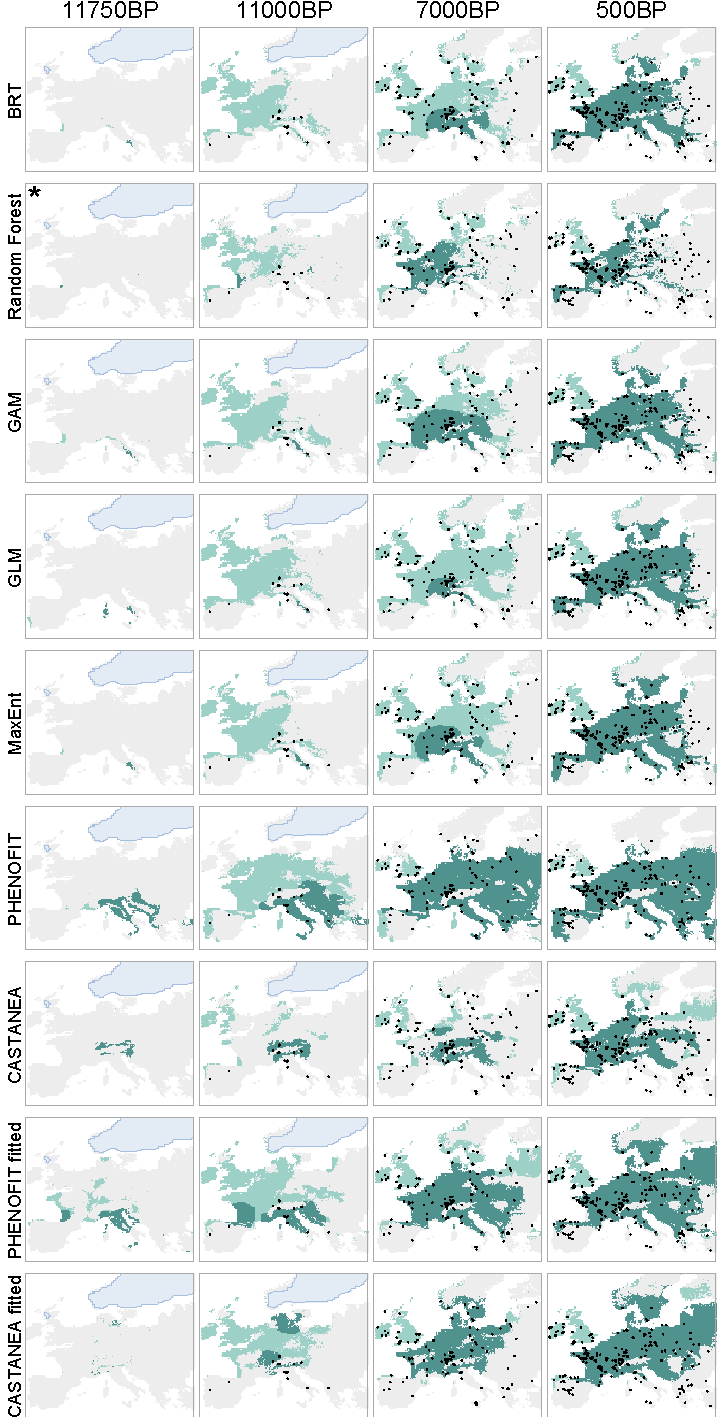
\includegraphics[width=0.7\linewidth]{chapter2/figs/quercus_deciduous_simulations.pdf}
\caption{\textbf{Example of paleosimulations obtained with the nine models used in this study for deciduous oaks.} The five first rows correspond to the five correlative models (boosted regression tree, down-sampled random forest, generalized additive model, generalized linear model with lasso regularization, MaxEnt). The four last rows correspond to two different versions (expert calibration and inverse calibration using occurrence data) of two explicit-based models (PHENOFIT and CASTANEA). Light green area is the modelled suitable area, dark green area is the colonized area (after migration). Light blue represents the ice sheet extent. Black dots are deciduous oak fossil pollen occurrences. The model for which migration started at 11.75 kyr BP rather than 12 kyr BP is marked with an asterisk. "BP" stands for "before present" (1950).}
\label{fig:quercusdeciduoussimulations}
\end{figure}

\subsection{Results}\label{results2}

As observed in previous long-term historical assessments, all models showed a decrease of their performance when moving further into the past, i.e. into more different climatic conditions than historical conditions (\Cref{fig:pastperformance}). However PEMs showed smaller decrease in their predictive performance (slope of Beta regression, fitted PEMs: $-6.07$, 95\% CI $[-8.62, -3.55]$, expert PEMs: $-4.44$, 95\% CI $[-7.07, -1.77]$) than CSDMs ($-11.0$, 95\% CI $[-13.2, -8.91]$). PEMs also showed higher transferability in the most distant climatic conditions of the early Holocene than CSDMs (\Cref{fig:pastperformance}). PEMs, either expert or fitted, are thus less affected by the increase in climate dissimilarity than CSDMs. In the near past (Late-Middle Holocene, $<$ 8.2 kyr BP), CSDMs were not significantly better at predicting tree distribution than any PEMs (pairwise Conover-Iman tests: \emph{vs.} expert PEMs \emph{t}-statistic $=1.68$/\emph{P} $=0.128$, \emph{vs.} fitted PEMs \emph{t}-statistic $=-1.55$/\emph{P} $=0.112$; \Cref{fig:pastperformance}), despite their closer fit to current species distributions (\Cref{fig:S8}). In the distant past (Early Holocene $>$ 8.2 kyr BP), CSDMs performed worse than both expert and fitted PEMs (pairwise Conover-Iman tests: respectively \emph{t}-statistic $=-4.80$/\emph{P} $<0.0001$ and \emph{t}-statistic $=-5.07$/\emph{P} $<0.0001$; \Cref{fig:pastperformance}). The maximum climatic dissimilarity during this period corresponds to the climatic dissimilarity expected as soon as 2060 according to the scenario SSP245 (\Cref{fig:pastperformance}).

These differences between PEMs and CSDMs are closely related to their ability to predict species recolonisation dynamics in the Early Holocene (\textappr11.5-8.5 kyr BP). Both types of PEMs, fitted and expert, predicted more accurately refugia locations at -12 kyr BP, which were the starting points for the migration (\Cref{fig:quercusdeciduoussimulations}; \hyperref[methods2]{Methods}). This period corresponds to a global deglaciation which lasted for a few centuries and occurred after the cooling of the Younger Dryas interval  (\textappr13-11.5 kyr BP; \Cref{fig:S1}). This rapid warming episode explains the strong decrease of climate dissimilarity relative to present between 12 kyr BP and 11.5 kyr BP (\Cref{fig:climaticdissimilarity}). If we had not considered the 12-11.5 kyr BP period of high climatic dissimilarity (i.e. without simulating migration from refugia), we would have missed the opportunity to take into account model projections within the same dissimilarity level to what we expect between 2050 and 2100 (\Cref{fig:climaticdissimilarity}). When models are compared after 11kyr BP, i.e. when climate dissimilarity is more similar to present, CSDMs and PEMs' abilities to predict fossil pollen occurrence are similar (\Cref{fig:S10}), with an average Sørensen index decrease of $-0.205\pm0.0224$ (paired Wilcoxon-test: \emph{P} $<0.0001$) between Late-Middle Holocene and Early Holocene.

Our results also revealed that inverse calibration improved process-explicit projections in recent past without altering significantly PEM long-term transferability (\Cref{fig:pastperformance}). In Middle-Late Holocene, when climate conditions were not drastically different from present, performances of fitted PEMs was higher than those of expert PEMs (\emph{t}-statistic $=2.70$/\emph{P} $=0.020$). In most distant climatic conditions of Early Holocene, their performances were similar (\emph{t}-statistic $=0.220$/\emph{P} $=0.757$; \Cref{fig:pastperformance}). 

Models performances were not stable across species, and exhibited both similarities and differences across time (\Cref{fig:S9}). More specifically, models exhibited the same overall performance decrease against \emph{Fagus} pollen records, whereas CSDM performance decline was substantially faster than expert and fitted PEMs for deciduous \emph{Quercus}. All models show low predictive power regarding evergreen \emph{Quercus} distribution even in the Late Holocene compared to other species, especially CSDMs which failed to predict its presence along the Atlantic coast (S6). Fitted PEMs, however, showed the lowest variability of performance across species (\Cref{fig:pastperformance}).

\subsection{Discussion}\label{disc}

Our results suggest that the transferability and robustness of models are more strongly influenced by the processes explicitly represented in the models than by their method of calibration. PEMs consistently show a better performance throughout the 12 kyr simulation period, even when calibrated using the same method as CSDMs (i.e. fitted PEMs). Therefore, beyond enabling a more detailed mechanistic understanding of the effects of environmental conditions on species survival, growth, and reproduction, biological processes represented in PEMs are also critical to ensure higher model robustness under more novel climatic conditions. This important new finding advocates for a wider use of PEMs to predict biodiversity and ecosystems distributions in the future and opens a new avenue to reach this goal by using inverse modelling approaches to calibrate them.

Our results also suggest that predictions of PEMs, either fitted or expert, should be more reliable at least up to 2060 according to the scenario SSP245 (\Cref{fig:pastperformance}) and 2050 according to SSP585. The rate of anthropogenic climate change and the increased probability of occurrence of novel climates (\Cref{fig:climaticdissimilarity}; \citealp{Williams2007}) are challenging the reliability of both CSDMs and PEMs especially since they are intended to be used in more complex models such as biosphere-atmosphere models and used by natural resource managers and policy makers to guide management plans and policies. Acknowledging these uncertainties is as important as making the forecasts themselves \citep{Beale2012} and contributes to the public trust in scientists \citep{Berkhout2010}.

\begin{figure}[ht!]
\hspace*{-0.6cm}
\centering
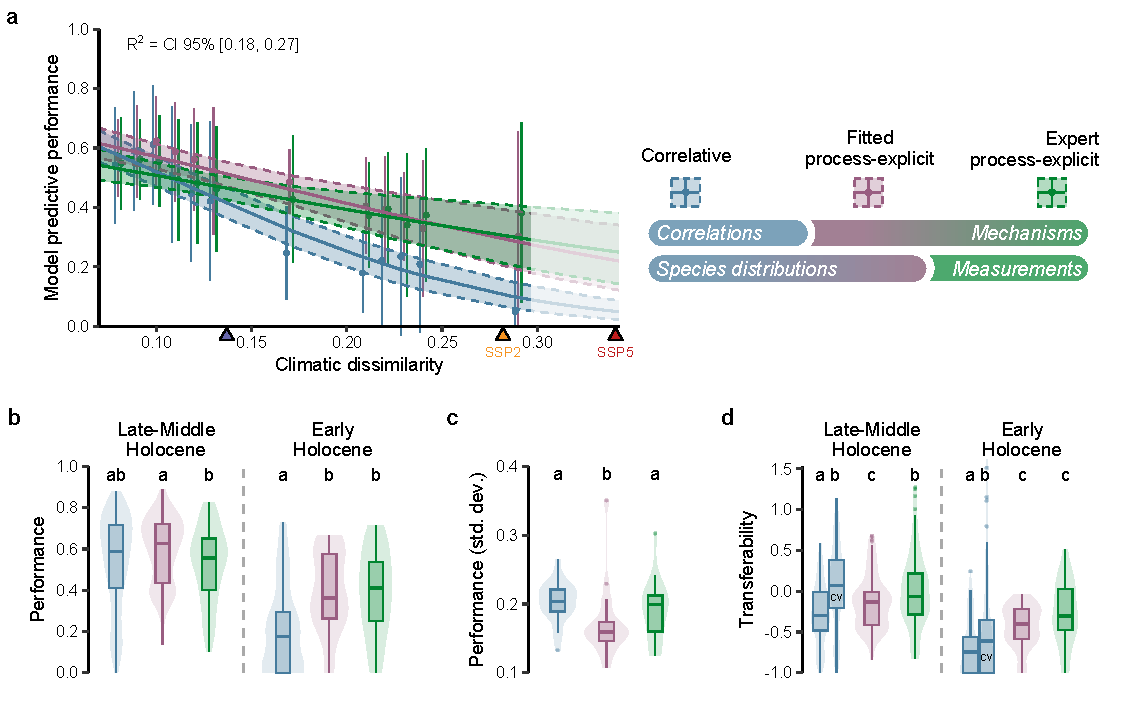
\includegraphics[width=17cm]{chapter2/figs/past_performance.pdf}
\caption{\textbf{Performance of correlative models, fitted process-explicit models (inverse calibration using occurrence data) and expert process-explicit models (classical calibration) against Holocene paleoecogical evidence (fossil pollen) for 4 tree genera (\emph{Abies}, \emph{Fagus}, \emph{Quercus} deciduous and \emph{Quercus} evergreen).} \textbf{(a)} Bayesian beta regression of model predictive performance (Sørensen index) against climatic dissimilarity relative to 1901-2000 (1-Sørensen similarity between climatic hypervolumes). Shaded areas represent 2.5\% and 97.5\% quantiles of the posterior predictive distribution. Points represent the average model performance (and lines the standard deviation) grouped by similar level of climatic dissimilarity. Blue triangle on x-axis indicates the limit between Early Holocene ($>$ 8.2 kyr BP) and Late-Middle Holocene ($<$ 8.2 kyr BP). Yellow and red triangles indicate the expected level of climatic dissimilarity in 2060 for SSP245 and SSP585 scenarios. Legend on the right: top row represents drivers of modelled distributions (correlations/mechanisms), bottom row represents calibration method (species distributions/measurements). Panels \textbf{(b)} and \textbf{(c)} show the difference in performance (Sørensen index) and variability in performance (standard deviation of Sørensen index) across models. Panel \textbf{(d)} shows the transferability of the models (relative change in model performance between distant past periods and historical period). A negative transferability means that model performance is lower in the distant past periods than in the historical period. CSDM predictive errors in the historical period was assessed by two different methods: (i) against the same data used for calibration (leading to an overestimation of historical model performance -- but more comparable to fitted PEM estimates), (ii) using an environmental block cross-validation, noted as "CV" (leading to a better estimation of true model errors in the historical period, and thus a higher transferability -- but less comparable to fitted PEMs for which cross-validation would have been too computationally expensive). The grouping letters represent the multiple comparisons with pairwise Conover-Iman tests.}
\label{fig:pastperformance}
\vspace*{1cm}
\end{figure}

Simulating migration allowed us to take into account the differences between the models under the most challenging conditions, i.e., when the climate dissimilarity was at its greatest, closely approximating what is projected for  the end of the 21\textsuperscript{st} century. Since the migration model is identical across all simulations, differences of performance between models across the Holocene very much depended on their ability to predict the potential refugia of the species during the Early Holocene. For example, some models were not able to predict evergreen \emph{Quercus} refugia in Southern Spain, thus missed an important migration route and failed predicting their presence in vast areas in the Late Holocene (\Cref{fig:S6}). As PEMs, either fitted or expert, describe the response of ecophysiological processes to a wide range of environmental conditions, they can provide a better estimate of the environmental conditions in which species could have survived 12000 years ago, under climates much more dissimilar to present conditions. A potential limitation of our approach though is that we cannot account for very rare and really long-distance dispersion events, as well as the influence of humans. For example all models failed to predict deciduous \emph{Quercus} in the British Isles before the Early Holocene sea level rise and the opening of the Strait of Dover (\Cref{fig:quercusdeciduoussimulations}; \citealp{Smith2011}), even though the land-sea mask changed throughout the simulations. It remains unclear whether this failure is due to the migration models' misrepresentation of very long-distance dispersion events of seeds (e.g. by humans or jays, across major dispersal barrier), or a consistent misprediction by both CSDMs and PEMs of more northern refugia.

The recent efforts to gather fossil pollen data and make them openly available \citep{Williams2018} allow us to objectively assess model performance under climate conditions vastly different from those used for their calibration. From 11.5 kyr BP onwards, climate dissimilarity varies between 0.29 and 0.08, a level equivalent to what we might experience in the second quarter of the 21\textsuperscript{st} century (\Cref{fig:climaticdissimilarity}). The  consistency of model projections with past observations does not demonstrate that model projections will be valid in the future \citep{Oreskes1994}, but making such comparisons allows to make a critical step towards enhancing our understanding of model transferability. As more and more pollen data becomes available, we could cover a wider range of conditions, notably prior 11.5 kyr BP. Our simulations nevertheless started at 12 kyr BP, when climatic dissimilarity was at its highest, and transitioned rapidly to a climate more analogous to historical state. The uncertainties on the initial conditions had thus a significant influence on the simulation outcomes. In the future, on the contrary, uncertainties on the initial conditions will be much lower as models will start from the known distributions of species, and uncertainties will increase as simulations proceed towards increasingly dissimilar climatic conditions, especially since these conditions  will extent beyond the range experienced in the past (\Cref{fig:S3}).

While quantifying the uncertainty in model projections remains challenging, our results pave the way for drastic improvement in model evaluation. The discrepancies between model performances we observed highlights the importance of considering various modelling methods to capture the full range of uncertainties associated with future projections. It implies that we should not rely solely on the model's own prediction dispersion to estimate projection uncertainties, nor on very similar modelling approaches, especially when climate dissimilarity sharply increases. Moreover, models will have to consider that tree colonization dynamics will likely be very different in the future because it will not only occur from a few refugia but from wider continuous ranges, and direct anthropogenic factors, such as land-use, sylvicultural practices and assisted species migration, will also shape the composition of forests \citep{Aitken2016, Guo2018, Ivory2019}.

Fitted PEMs bring together the strengths from both CSDMs and expert PEMs approaches by describing causal relationships between environmental conditions and species performance (i.e. from process-explicit approaches) and precise estimates of parameter values (from correlative approaches). The differences between expert and fitted PEMs in the Middle-Late Holocene pinpoint some issues in expert parameterization that requires to combine various methods to cope with both the scarcity of data for each ecophysiological process modelled and sometimes non-measurable parameters \citep[e.g.][]{DeCaceres2023}.  Some parameters in these relations can be measured directly, and exhibit little variability across a species range (e.g. water potential leading to 50\% of vessels embolism). However, the measurement of parameters in controlled conditions does not necessarily guarantee their external validity \emph{in natura} \citep{Asse2020} where numerous factors, not represented in laboratory conditions, can also affect the process modelled \citep[but see][]{Satake2013}. Other parameters are in addition either highly variable because of local adaptation over long period,  difficult-to-measure or so far unmeasurable (e.g. bud dormancy). Therefore, expert PEMs can suffer from uncertainties entailed in the measurements of some of their parameters, and from spurious data specific to few locations which do not represent sufficiently well all the conditions the species can experience all over its range. For these reasons, inverse calibration presents a valuable opportunity to estimate the values of PEM parameters especially difficult to estimate otherwise \citep{Evans2016, Hartig2014}. However, inverse calibration does not warranty the correct estimation of parameter values and needs to be used critically and with caution \citep{VanderMeersch2023}. 

Our unique multi-model comparison across the Holocene demonstrates that our understanding of biological mechanisms embedded into process-explicit models represent a real advantage over the empirical relationships used in CSDMs to increase projections reliability for the coming decades. However, data availability limits our ability to parameterize these models, and could explain the difficulty to use them more widely for global impact studies. Fitted PEMs may overcome this problem by using more data at a larger geographical scale, while keeping the predictive strength of causal relationships. Given ongoing improvements in computational methods and the availability of new global-scale measurements (e.g. forest structure and growth with remote sensing and LiDAR data), extensive calibration and more widespread application of process-explicit models seems now possible as well as an increase in model projections reliability.

\clearpage

\subsection{Acknowledgements}
The authors are deeply grateful for many helpful comments from Elizabeth M. Wolkovich, which have greatly enriched this manuscript. They would also like to thank Christophe Randin for his valuable input throughout the course of this research, Jed O. Kaplan for making GWGEN and LPJ-LMfire codes openly available, as well as Sandy Harrison and Colin Prentice for interesting discussions on this work. They acknowledge the support and computing resources of GenOuest and TGCC-CEA. \\
Future climate scenarios used were from the NEX-GDDP-CMIP6 dataset, prepared by the Climate Analytics Group and NASA Ames Research Center using the NASA Earth Exchange and distributed by the NASA Center for Climate Simulation (NCCS). They acknowledge the World Climate Research Programme, which, through its Working Group on Coupled Modeling, coordinated and promoted CMIP6. \\
V.V. was supported by a PhD Fellowship from the GAIA doctoral school of the University of Montpellier, France.

\subsection{Author contributions}
\textbf{V.V.}: Conceptualization, Methodology, Investigation, Analysis, Writing - Original Draft, Writing - Review \& Editing. \textbf{E.A.}: Resources, Writing - Review \& Editing. \textbf{F.M.}: Methodology, Writing - Review \& Editing. \textbf{A.D.}: Writing - Review \& Editing. \textbf{H.D.}: Methodology, Writing - Review \& Editing. \textbf{F.S.}: Conceptualization, Writing - Review \& Editing. \textbf{I.C.}:  Conceptualization, Methodology, Writing - Review \& Editing, Supervision.

\subsection{Data availability}
Simulation outputs, together with the code to reproduce the analysis and figures in this study, are available on GitHub at \url{https://github.com/vvandermeersch/past_robustness}.